\documentclass[conference]{IEEEtran}
%\usepackage{a4wide}
\usepackage{NotationStyle}
\usepackage[ruled, vlined]{algorithm2e}
\usepackage{multicol, multirow}
%\usepackage[noend]{algorithmic}
\usepackage[english]{babel}
\usepackage{amsmath,amssymb,mathrsfs,mathtext}
\usepackage{subfig}
\usepackage{graphics,graphicx,epsfig}
\usepackage{epstopdf}
\usepackage{fancybox,fancyhdr}
\usepackage{enumerate}
\usepackage{array}
\usepackage{color, soul}
%\usepackage{longtable} % longtable doesn't work with two columns
\usepackage{supertabular}
\usepackage[normalem]{ulem}
\usepackage{arydshln}
%\usepackage{accents} % for the sake of doublehat!
%\newlength{\dhatheight}
%\newcommand{\doublehat}[1]{%
%    \settoheight{\dhatheight}{\ensuremath{\hat{#1}}}%
%    \addtolength{\dhatheight}{-0.35ex}%
%    \hat{\vphantom{\rule{1pt}{\dhatheight}}%
%    \smash{\hat{#1}}}}


%\makeatletter
%\let\oldlt\longtable
%\let\endoldlt\endlongtable
%\def\longtable{\@ifnextchar[\longtable@i \longtable@ii}
%\def\longtable@i[#1]{\begin{figure}[t]
%\onecolumn
%\begin{minipage}{0.5\textwidth}
%\oldlt[#1]
%}
%\def\longtable@ii{\begin{figure}[t]
%\onecolumn
%\begin{minipage}{0.5\textwidth}
%\oldlt
%}
%\def\endlongtable{\endoldlt
%\end{minipage}
%\twocolumn
%\end{figure}}
%\makeatother

\setlength\dashlinedash{0.2pt}
\setlength\dashlinegap{4.5pt}


\newcommand{\argmax}{\mathop{\rm arg\,max}\limits}
\graphicspath{ {../code/fig/} {fig/} {../code/}}

\renewcommand{\baselinestretch}{1.3}
\begin{document}
\title{Feature generation for multiscale time series forecasting}



%Radoslav Neychev, Eric Gaussier and Vadim Strijov}
\date{Technical report (pre-draft)}
\maketitle

\begin{abstract}
The paper presents a framework for the multiscale time series forecast. We reduce the problem of time series forecast to the regression problem and propose a method of constructing efficient feature description for the regression problem.
The method involves feature generation, followed with dimensionality reduction procedure. Generated features include historical information about the target time series as well as other available time series, local transformations and  multiscale features. We apply several forecasting algorithms to the resulting regression problem and investigate the quality of the forecasts for various horizon values.
\end{abstract}



\section{Introduction}
The paper investigates behavior of a device within the concept of Internet of Things. The device at question is monitored by a set of sensors, which produces large amount of multi-scale time series during its lifespan. These time series have various time scales since distinct sensors produce observations with various frequencies (milliseconds, days, weeks, etc).  The main goal is to forecast the observations of a device in a given time range.

We assume that the sampling rate of each time series is fixed and each time series has its own forecast horizon. The problem of multi-scale analysis arises in such applications as weather prediction, medical diagnosis and monitoring various sensor time series~\cite{Costa2008, Ahmed2012, Cortez2012, Ferreira2006} \hl{[medical, medical, traffic, ecology]}. Motivation for multi-scale analysis comes from the assumption that the behaviour of complex signals may be governed by  essentially different processes at various time scales. Thus, the time series should be modeled separately at each scale. This approach is used in time series classification, prediction and fault detection~\cite{Cui2016, Cortez2012, Aldrich2013}. Regardless of the goal of multi-scale analysis, it includes sequential averaging of the time series to obtain more coarse-scaled time series~\cite{Wu2013}, or, more rarely, differencing the time series for a more detailed, fine-scaled version of the time series~\cite{Jiang2011}. Averaging and differencing, which is equivalent to application of Haar's wavelet transform~\cite{Jiang2011}, may be replaced by any other pair of low and high pass wavelet filters~\cite{Chen2004} or convolution operation with some kernel function~\cite{Vespier2012}. Next steps depend on the goal of multi-scale analysis. Using multi-scale approach in time series prediction usually involves determining optimal scales~\cite{Vespier2012, Ahmed2012}, decomposition of time series into separately forecasted components and combination of the obtained forecasts.


\section{Related work}
 Along with generic methods of time series forecasting, such as Autoregressive Moving Average Models (ARMA), Autoregressive Integrated Moving Average Models (ARIMA), many authors report high predictive performance of the methods, originally developed for classification or regression, applied to forecast time series. The latter include Support Vector Regression~\cite{Trafalis2000, Navarrete2015, Hao2006}, random forests~\cite{Yu2016, Kane2014} and artificial neural networks~\cite{Busseti2012, Taylor2009}.
 %The authors of~\cite{Trafalis2000, Hao2006} reported high predictive performance of SVR applied to time series forecasting.
 Random Forests combine decision trees with randomly generated nodes to increase the accuracy of classification or regression~\cite{Criminisi2011}. In case of regression trees, each node of the tree splits the input space into two subspaces and each leaf specifies a distinct regression model, which is used for prediction if the input is found in the corresponding region of the input space. Predictions of the trees in the forest are averaged, or, for the probabilistic random forest, the probabilities of the outputs are averaged. The advantage of random forests is their efficiency in case of highly dimensional data due to the randomness incorporated into selecting informative features. Since random forests are essentially ensembles of weak learners, they enjoy high generalization ability, associated with boosting algorithms. The authors of~\cite{Criminisi2011} compare regression with probabilistic Random Forest with

 Here the input variables are the delayed observations  of the time series, and the output is the forecasted value of time series. However, the authors of~\cite{Navarrete2015} show that this prediction framework suffers from systematic error that does not converge to zero as the sample size increases, since both the inputs and the outputs are noised and regression algorithms do not handle the noise in the input correctly. To ensure error convergence, the authors first apply cubic spline approximation, which yields much lower RMSE in case of noisy data. The impact of spline approximation is not so great when the noise is low or discretization is too coarse.

 To extend this one-step-ahead forecasting scheme to the case of multiple predictions, one may use iterative, direct or multiple output strategies~\cite{Bao2014}. Within the iterative strategy, one-step-ahead forecasts are computed recursively, with the newly predicted values of the time series used as the actual future records. A less prone to error accumulation, though more time consuming method is the direct strategy, which involves estimation of $h$ models to predict $h$ future values of the time series~\cite{Zhang2013}. Finally, the multiple input multiple output (MIMO) strategy allows to obtain $h$ prediction with at one step. In case of SVR, MIMO strategy is based on multivariate SVR~\cite{PerezCruz2002}. The paper~\cite{Bao2014} compares different strategies of multi-step-ahead prediction in SVR-based forecasting: direct, iterative and multiple output. Regardless of the horizon values, direct and MIMO strategies consistently achieve more accurate forecasts, than the iterative strategy, with MIMO being most accurate in most cases.

Additionally, there are multiple suggestions on how to combine these forecasting methods~\cite{Qiu2014, Grover2015} or use them in the multi-scale fashion~\cite{Chen2004, Zhu2012, Cui2016, Bai2015, Ferrari2012}.


\section{Problem statement}
Consider a large set of time series~$\fD=\{\bs^{(m)}| \; m = 0\dots, {M}\}$, where each real-valued time series~$\bs$
\[ \bs = [s_1, \dots, s_i, \dots, s_{T}], ~~ s_i = s(t_i),\quad 0 \leq t_i \leq t_{\max}\]
is a sequence of observations $s_i = s(t_i)$ of some real-valued signal $s(t)$\footnote{The signal s(t) and the resultant time series $\bs$ are potentially multivariate. We use the same notation for multivariate and univariate time series. }.
Each time series $\bs^{(m)}$ has its own sampling rate $1/\tau^{(m)}$:
\[t_i^{(m)} = {i}\cdot\tau^{(m)}.\]

 The task is to obtain forecasts $\hat{s}^{(0)}(t_i)$ for  $\dtr <  t_i \leq T_{\max} + \dtr$, given the set  $\fD$. (Fig.~\ref{fg:online_frc}), which minimise mean absolute percentage errors~\ref{fg:retrospective}
% \begin{equation}\label{eq:forecasting_problem}
% \end{equation}
 \[ MAPE(\bs, \hat{\bs}) = \frac{1}{r}\sum_{i = 1}^{r} \frac{|s_i - \hat{s}_i|}{|s_i|}. \]
Here MAPE is evaluated for the retrospective forecasts~\ref{fg:retrospective}, where the most recent historical samples $\bx_0^{*}$ are concealed and forecasted as if they were unknown. Then the quality of the model $\fx$ is evaluated according to its performance on these concealed samples.


 We consider the forecasting problem as the multivariate regression problem, where target variables are the vectors of lagged values $s^{(0)}(t_i)$ of the target time series $\bs^{(0)}$. form an object set at a set Let $\bx^{*}$ denote rows of the design matrix for the regression problem. Each vector~$\bx^{*} = [\by| \bx]$ collects all the time series over the time period~$\dtp$ (Fig.~\ref{fg:draw}), which stands for the local \emph{prehistory}. The vector $\bx^{*}$ includes samples from previous history of time series from $\fD$ as well as any derivatives $\vf$, which are called generated features.



\begin{figure}[!ht]
\centering
\subfloat[]{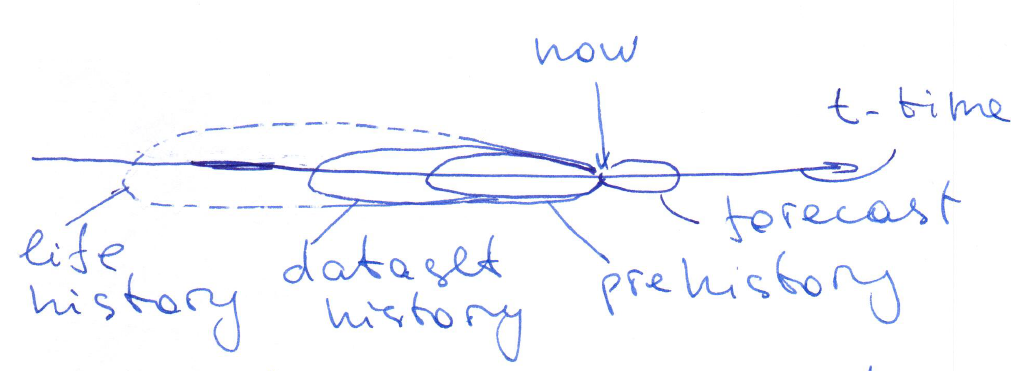
\includegraphics[width=0.4\textwidth]{online_forecasting_paradigm.png}
\label{fg:online_frc}} \\
\centering \subfloat[]{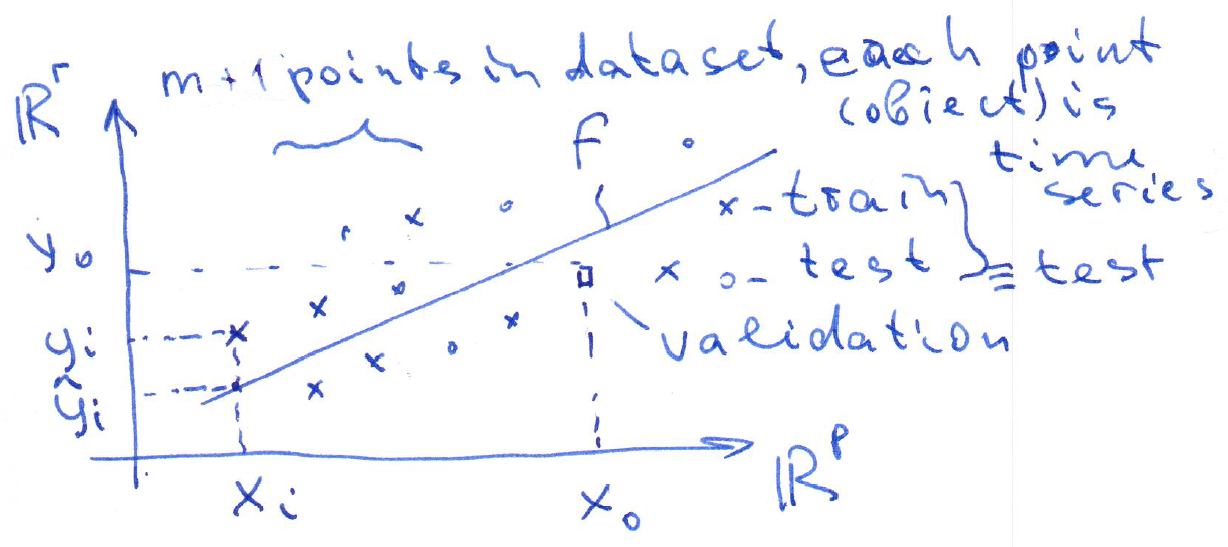
\includegraphics[width=0.4\textwidth]{forecasting_model.png}
\label{fg:forecasting}
}
\caption{Forecasting (a) as regression problem (b).}
\end{figure}

\subsection{Design matrix}

\begin{figure}[!ht]
\centering
\subfloat[]{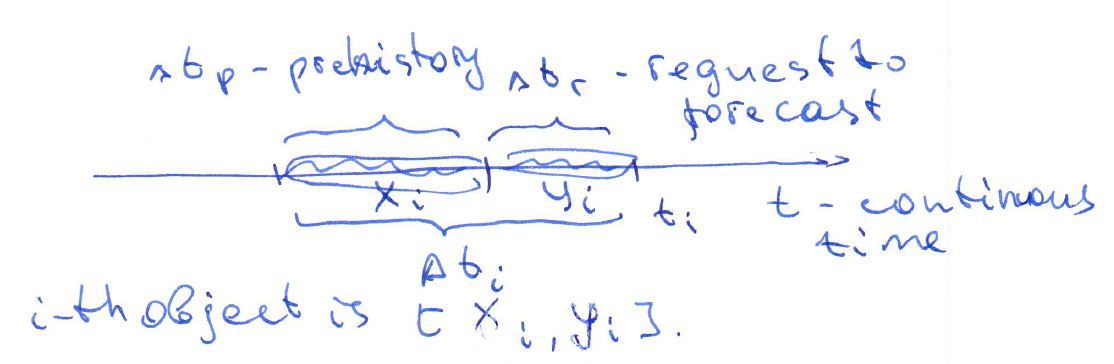
\includegraphics[width=0.4\textwidth]{draw_object.png}\label{fg:draw}} \\
\centering\subfloat[]{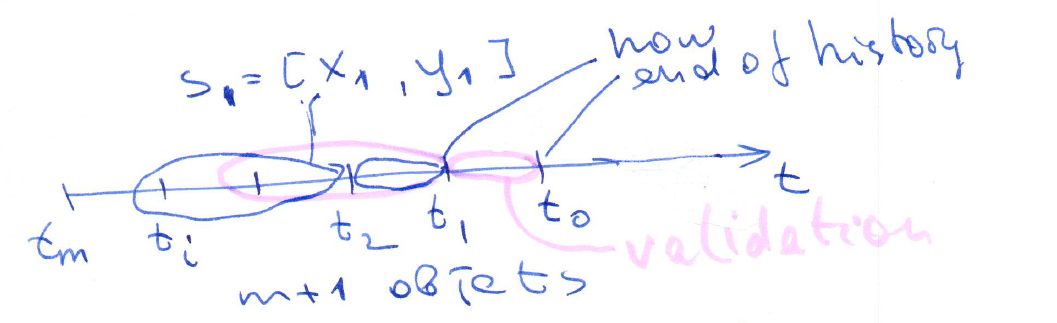
\includegraphics[width=0.4\textwidth]{design_matrix_generation.png}\label{fg:design}}
\caption{Draw an object from time series history.}
\end{figure}

The design matrix~$\bX^*$ for the multiscale autoregressive problem statement is constructed  as follows (Fig.~\ref{fg:design}). Let $\bs^{(m)}_i$ denote the~$i$-th segment of the time series $\bs^{(m)}$
\begin{equation}\label{eq:segment}
[\bx^{(m)}_i | \by^{(m)}_i] = \end{equation}
\[ \underbrace{s^{(m)}(t_i-\dtr-\dtp),\dots,}_{\bx^{(m)}_i} \underbrace{s^{(m)}(t_i-\dtr),\dots,s^{(m)}(t_i))}_{\by^{(m)}_i}], \]

where~$s^{(m)}(t)$ is an element of time series~$\bs^{(m)}$. To construct the design matrix, select $t_i$, $i = 1, \dots, q$ from $\Gs = \{t_1, \dots, t_T\}$ such that segments $\bs_i = [\x_i|\y_i]$ cover time series $\bs$
%\begin{equation}\label{eq:strategy2} \{s(t_{1}), \dots, s(t_{\max})\} = \bigcup_{i=1}^{q-1} \{s(t_i-\Delta t_\text{r}),\dots,s(t_i)\}\end{equation}
without intersection in target parts  $\y_i$:
\begin{equation}\label{eq:strategy2} |t_{i+1} - t_i| > \dtr.
\end{equation}
Following~\eqref{eq:segment} and~\eqref{eq:strategy2}, extract segments $[\bx^{(m)}_i | \by^{(m)}_i]$, $i = 1, \dots, q$ from all time series $\bs^{(m)} \in \fD$ and form the matrix
 \begin{equation}\label{eq:design_matrix}
\bX^*= \left[
\begin{array}{c|c}
 \underset{q{\times}n}\bX & \underset{q{\times}r}\bY  \\
 \hline
 \underset{1{\times}n}{\x} & \underset{1{\times}r}{{\by}}  \\
\end{array}
\right] = \left[
\begin{array}{llll|l}
\bx_1^{(0)} & \bx_1^{(1)}  & \dots & \bx_1^{(M)} & \by_1^{(0)}   \\
\vdots & \vdots & \ddots & \vdots & \vdots   \\
\bx_q^{(0)} &  \bx_q^{(1)} & \dots & \bx_q^{(M)} & \by_q^{(0)}   \\

\hline
\bx^{(0)} &  \bx^{(1)} & \dots & \bx^{(M)} &  {\by}^{(0)}   \\
\end{array}
\right]. \end{equation}

Denote a row from the pair~$\bY,\bX$ as $\by,\bx$ and call these vectors the target and the features.

\begin{figure}[!ht]
\centering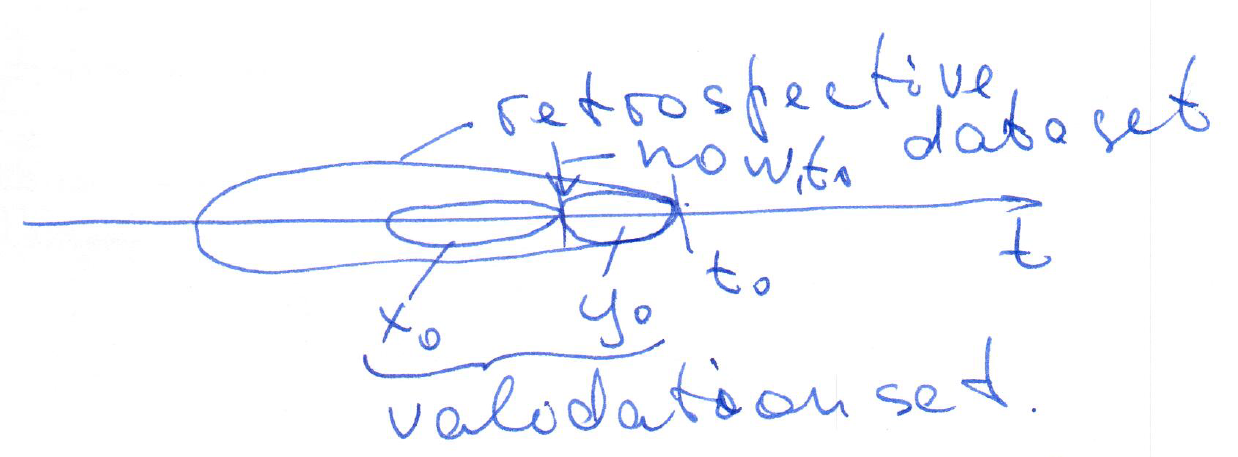
\includegraphics[width=0.4\textwidth]{retrospective_validation.png}
\caption{\hl{Retrospective forecast includes most recent samples in data set.}\label{fg:retrospective}}
\end{figure}

Now we are able the regression problem as follows:
\begin{equation}\label{eq:regression_problem}
\hat{\y} = f(\x, \hat{\w}), \text{~where~}
\end{equation}
\[ \hat{\w} = \argmin_{\hat{\w}}\frac{r}{q}\sum_{i=1}^{q} MAPE(\y_i, f(\x_i, \w)).\]

\section{Feature generation}
The feature set $\mathcal{J} = \mathop{\cup}\limits_k \mathcal{A}_k$ includes
\begin{enumerate}[1)]
\item the local history of all time series themselves,
\item transformations (non-parametric and parametric) of local history,
\item parameters of the local models,
\item distances to the centroids of local clusters.
\end{enumerate}


Denote the generated feature vector as~$\vf$. This vector consists of concatenated row-vectors~$\vf=[\vf^{(1)},\dots,\vf^{(M)}]$, which corresponds to time series local histories ~$\bs=[\bs^{(1)},\dots,\bs^{(M)}]$, modified with set of transformations~$\mathfrak{G}$. The elements~$g:\bs\to\vf$ of this set are listed below.

\subsection{Transformations of local history}
The tables~\ref{tb:musttries},~\ref{tb:elementaries},~\ref{tb:monotones},~\ref{tb:multivariates},~\ref{tb:datastats} list the~time series transformation functions. There are non-parametric and parametric procedures to generate features. For the parametric functions~$g=g(\bb,s)$ the default values of the parameters~$\bb$ are assigned empirically.

The parametric procedure request two optimization problem statements of the model parameters~$\bw$ and the primitive function parameters~$\bb$. The first one fixes the vector~$\hat\bb$, collected over all the primitive functions~$\{g\}$, which generate features~$\vf$:
\[
\hat\bw = \arg\min S\bigl(\bw|\fx(\bw,\bx),\by\bigr),\quad
\text{where}
\quad [\by,\bx] = \vf(\hat\bb,\bs).
\]
The second one optimizes the transformation parameters~$\hat\bb$ given obtained model parameters~$\bw$
\[
\hat\bb = \arg\min S\bigl(\bb|\fx(\hat\bw,\bx),\by\bigr).
\]
This procedure repeats two problems until vectors~$\hat\bw,\hat\bb$ converge. \hl{The initial values of vector~$\bb$ (are shown in table}~\ref{tb:primitives}). Due to the various origins of the time series and their transformations the residual vector should be normalized:
\[\veps = \frac{\hat\by-\by}{|\by| \cdot \|\by\|_2^1}.
\]
\hl{It (transformation? normalization)} does not change the number elements in the vectors,~$|\vf|=|\bs|$.

\subsection{Convolutions, statistics and parameters of local history}
The listed feature generation functions convolves time series, so they reduce the dimensionality $|\vf=\bg(\bs)|<|\bs|$.

\subsection{Parameters of local history forecast}
For the time series~$\bs$ construct the Hankel matrix with a~period~$k$ and shift~$p$, so~that for~$\bs = [s_1,\dots,s_T]$ the matrix
\[
\bH^* =
\left[ \begin{array}{c|cc}
s_T  & \dots & s_{T-k+1} \\
\vdots & \ddots & \vdots \\
s_{k+p} & \dots & s_{1+p}\\
s_k & \dots & s_1 \\
\end{array}
\right],
\text{~where~} 1\geqslant p \geqslant k .
\]
Reconstruct the regression to the first column of the matrix~$\bH^*=[\bh, \bH]$ and denote its least square parameters as the feature vector
\[
\boldsymbol{\phi}^{(m)} = \arg\min \| \bh-\bH \boldsymbol{\phi}\|_2^2.
\]
For the time series~$\bs^{(m)}$, $m=1,\dots, M$ use the parameters $\boldsymbol{\phi}^{(m)}$ as the features.

\subsection{Distances to centroids of local clusters}
This procedure applies the kernel trick to the time series. For given local history time series~$\bx_i^{(m)}$, $m=1,\dots, M$ compute $k$-means centroids~$\bc_p^{(m)}$, $p = 1, \dots, P$.  With the selected $k$-means distance function~$\rho$ construct the feature vector
\[
\vf_i^{(m)} = [\rho(\bc_1^{(m)},\bs_i^{(m)}),\dots,\rho(\bc^{(m)}_P,\bs_i^{(m)})] \in \R_+^P.
\]
This $k$-means of another clustering procedure may use internal parameters, so that there are no parameters to be included to the feature vector or to the forecasting model.



\section{Feature selection}
TODO



\section{Computational experiment}
The goal of the experiment is to study the performance of multivariate regression approach to the problem of
time series forecasting.

This section presents the results of computational comparison of the forecasting models presented above. To test each model, we used several datasets, described below.

\paragraph{Datasets}
\begin{itemize}
\item Energy consumption dataset. The dataset consists of the Polish electricity load time series~\cite{EnergyWeatherData} and weather time series in Warsaw (Longtitude: 21.25, Latitude: 52.30, Elevation: 94). Energy time series contain hourly records, weather time series were measured daily. The dataset comprises two original time multiscale series, which correspond to the periods of 1999--2001 and 2002-2004 and is augmented with artificially modified versions of these two time series. \hl{More on data preparation.}
\item Accelerometry dataset. This dataset consists of accelerometry time series from the Human Activity Sensing Consortium~\cite{HASCdata}. Each time series in the datasets is a sequence of acceleration records. The time series were recorded for 120 seconds while a subject performed a sequence of activities: stay, walk, jog, skip, stair up or stair down. The sampling rate varies between 10 and 100Hz, but stays constant for each time series.
\item Financial dataset~\cite{NNcompetition}.  The dataset A (final, complete) from the 2006/07 Forecasting Competition for Neural Networks \& Computational Intelligence. The dataset contains 111 monthly time series drawn from homogeneous population of empirical business time series.
\end{itemize}

\paragraph{Experimental results}
Each time series from the datasets was converted to the design matrix~\eqref{eq:design_matrix} and used as input data to train regression models according to~\eqref{eq:regression_problem}.

Table~\ref{fg:feature_selection_res_HASC1} lists forecasting errors for the proposed feature generation strategies applied to the test time series from the HASC dataset.

Fig.~\ref{fg:target_data} displays an example of target time series HASC1001 and the results of forecasting a single segment of this time series with the baseline models.

Fig.~\ref{fg:feature_gen_frc} illustrates the results of regression built on the design matrix, augmented with the particular data generation method.

Fig.~\ref{fg:pca_frc} demonstrates the forecasts, obtained by each model in the proposed framework. Here the design matrix was augmented with the generated features and PCA was applied to select a subset of features.



\begin{figure}[!t]
\centering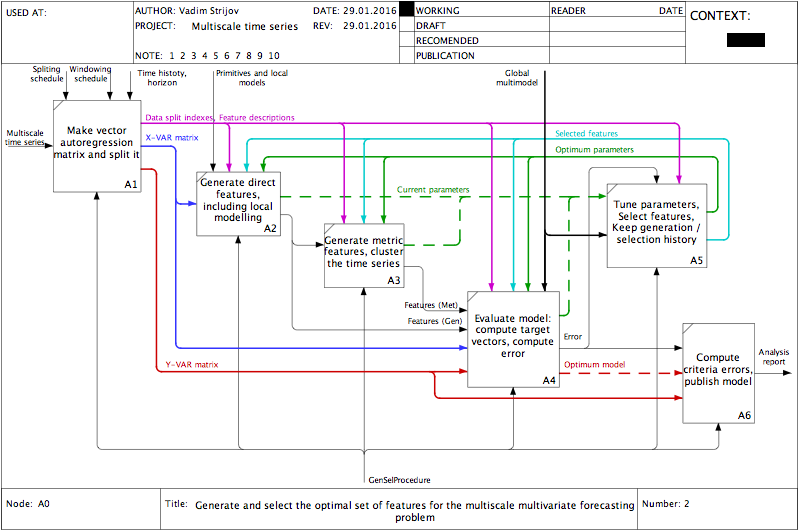
\includegraphics[width=0.45\textwidth]{02_A0.png}
\label{fg:IDEF}
\caption{Multiscale forecasting pipeline.}
\end{figure}


\begin{table}
\begin{tabular}{|c|c|c|c|c|}
\hline
Feature set & Models &MAPE test & MAPE train & AIC\\
\hline
\multirow{4}{*}{History} &VAR &   7.215 &    0.067 &    1427.927\\
\cline{2-5}
 &SVR &   0.718 &    0.320 &    1396.463\\
\cline{2-5}
 &Random Forest &   0.463 &    0.206 &    1388.668\\
\cline{2-5}
 &Neural network &   0.624 &    0.407 &    1389.319\\
\cline{2-5}
\hline
\multirow{4}{*}{SSA} &VAR &   0.755 &    0.402 &    1375.959\\
\cline{2-5}
 &SVR &   1.348 &    0.434 &    1401.053\\
\cline{2-5}
 &Random Forest &   0.746 &    0.335 &    1413.181\\
\cline{2-5}
 &Neural network &   0.544 &    0.387 &    1379.299\\
\cline{2-5}
\hline
\multirow{4}{*}{Cubic} &VAR &   0.562 &    0.382 &    1371.387\\
\cline{2-5}
 &SVR &   0.779 &    0.418 &    1373.299\\
\cline{2-5}
 &Random Forest &   0.647 &    0.320 &    1412.390\\
\cline{2-5}
 &Neural network &   0.795 &    0.387 &    1371.354\\
\cline{2-5}
\hline
\multirow{4}{*}{Conv} &VAR &   2.182 &    2.180 &    2252.866\\
\cline{2-5}
 &SVR &   2.986 &    0.537 &    1413.103\\
\cline{2-5}
 &Random Forest &   0.583 &    0.323 &    1408.932\\
\cline{2-5}
 &Neural network &   0.743 &    0.406 &    1373.955\\
\cline{2-5}
\hline
\multirow{4}{*}{NW} &VAR &   2.021 &    0.041 &    1605.095\\
\cline{2-5}
 &SVR &   0.714 &    0.323 &    1398.156\\
\cline{2-5}
 &Random Forest &   0.427 &    0.195 &    1381.996\\
\cline{2-5}
 &Neural network &   0.815 &    0.425 &    1389.418\\
\cline{2-5}
\hline
\multirow{4}{*}{All} &VAR &   2.000 &    2.000 &    9910.259\\
\cline{2-5}
 &SVR &   0.751 &    0.324 &    1395.951\\
\cline{2-5}
 &Random Forest &   0.415 &    0.194 &    1381.906\\
\cline{2-5}
 &Neural network &   1.254 &    0.399 &    1381.405\\
\cline{2-5}
\hline
\multirow{4}{*}{PCA} &VAR &   0.712 &    0.310 &    1388.756\\
\cline{2-5}
 &SVR &   0.748 &    0.323 &    1395.828\\
\cline{2-5}
 &Random Forest &   0.504 &    0.214 &    1378.500\\
\cline{2-5}
 &Neural network &   0.563 &    0.392 &    1377.608\\
\cline{2-5}
\hline
\end{tabular}
\caption{Forecasting errors measured as symmetric MAPE.}
\label{fg:feature_selection_res_HASC1}
\end{table}


\begin{figure}
\centering
%\subfloat[]{\includegraphics[width=0.18\textwidth]{fig/feature_selection/HascData/data_HASC1001.png}}
\subfloat[]{\includegraphics[trim= 2cm 0 0 15cm,clip,width=0.25\textwidth]{fig/feature_selection/HascData/data_segms_HASC1001.png}}
\subfloat[]{\includegraphics[trim= 2cm 0 0 15cm,clip,width=0.25\textwidth]{fig/feature_selection/HascData/res_HASC1001.png}}
\caption{Accelerometry time series from HASC project.
(a) Target segments of the time series HASC1001. (b) Forecasting results for	HASC1001 (VAR, SVR, Random Forest, Neural network).}\label{fg:target_data}
\end{figure}


\begin{figure}
\centering
\subfloat[VAR]{\includegraphics[trim= 2cm 0 0 15cm,clip, width=0.25\textwidth]{fig/frc_analysis/HascData/stats_HASC1001VAR.png}}
\subfloat[SVR]{\includegraphics[trim= 2cm 0 0 15cm,clip,width=0.25\textwidth]{fig/frc_analysis/HascData/stats_HASC1001SVR.png}}\\
\subfloat[Random forest]{\includegraphics[trim= 2cm 0 0 15cm,clip, width=0.25\textwidth]{fig/frc_analysis/HascData/stats_HASC1001Random_Forest.png}}
\subfloat[ANN]{\includegraphics[trim= 2cm 0 0 15cm,clip, width=0.25\textwidth]{fig/frc_analysis/HascData/stats_HASC1001Neural_network.png}}\\
\caption{Mean residual by number of forecasted point.}
\end{figure}

\begin{figure}
\centering
\subfloat[VAR]{\includegraphics[trim= 2cm 0 0 15cm,clip, width=0.25\textwidth]{fig/frc_analysis/HascData/npdf_HASC1001VAR.png}}
\subfloat[SVR]{\includegraphics[trim= 2cm 0 0 15cm,clip,width=0.25\textwidth]{fig/frc_analysis/HascData/npdf_HASC1001SVR.png}}\\
\subfloat[Random forest]{\includegraphics[trim= 2cm 0 0 15cm,clip, width=0.25\textwidth]{fig/frc_analysis/HascData/npdf_HASC1001Random_Forest.png}}
\subfloat[ANN]{\includegraphics[trim= 2cm 0 0 15cm,clip, width=0.25\textwidth]{fig/frc_analysis/HascData/npdf_HASC1001Neural_network.png}}\\
\caption{Normal probability density functions fitted to residuals of each model.}
\end{figure}

\begin{figure}
\centering
\subfloat[VAR]{\includegraphics[trim= 2cm 0 0 15cm,clip, width=0.25\textwidth]{fig/frc_analysis/HascData/qq_HASC1001VAR.png}}
\subfloat[SVR]{\includegraphics[trim= 2cm 0 0 15cm,clip,width=0.25\textwidth]{fig/frc_analysis/HascData/qq_HASC1001SVR.png}}\\
\subfloat[Random forest]{\includegraphics[trim= 2cm 0 0 15cm,clip, width=0.25\textwidth]{fig/frc_analysis/HascData/qq_HASC1001Random_Forest.png}}
\subfloat[ANN]{\includegraphics[trim= 2cm 0 0 15cm,clip, width=0.25\textwidth]{fig/frc_analysis/HascData/qq_HASC1001Neural_network.png}}\\
\caption{Quantile-quantile plots for each model.}
\end{figure}

\begin{figure}
\centering
\subfloat[SSA]{\includegraphics[trim= 2cm 0 0 15cm,clip, width=0.25\textwidth]{fig/feature_selection/HascData/res_HASC1001_fs_SSA.png}}
\subfloat[Cubic]{\includegraphics[trim= 2cm 0 0 15cm,clip, width=0.25\textwidth]{fig/feature_selection/HascData/res_HASC1001_fs_Cubic.png}} \\
\subfloat[Conv]{\includegraphics[trim= 2cm 0 0 15cm,clip, width=0.25\textwidth]{fig/feature_selection/HascData/res_HASC1001_fs_Conv.png}}
\subfloat[NW]{\includegraphics[trim= 2cm 0 0 15cm,clip, width=0.25\textwidth]{fig/feature_selection/HascData/res_HASC1001_fs_NW.png}} \\
\subfloat[All]{\includegraphics[trim= 2cm 0 0 15cm,clip, width=0.25\textwidth]{fig/feature_selection/HascData/res_HASC1001_fs_all.png}}
\subfloat[PCA]{\includegraphics[trim= 2cm 0 0 15cm,clip, width=0.25\textwidth]{fig/feature_selection/HascData/res_HASC1001_fs_pca.png}} \\
\caption{Forecasting results for various feature generation strategies, HASC1001.}\label{fg:feature_gen_frc}
\end{figure}


\begin{figure}
\centering
\subfloat[VAR]{\includegraphics[trim= 2cm 0 0 15cm,clip, width=0.25\textwidth]{fig/feature_selection/HascData/res_HASC1001_VAR_fs_pca.png}}
\subfloat[SVR]{\includegraphics[trim= 2cm 0 0 15cm,clip, width=0.25\textwidth]{fig/feature_selection/HascData/res_HASC1001_SVR_fs_pca.png}}\\
\subfloat[Random Forest]{\includegraphics[trim= 2cm 0 0 15cm,clip, width=0.25\textwidth]{fig/feature_selection/HascData/res_HASC1001_Random_Forest_fs_pca.png}}
\subfloat[ANN]{\includegraphics[trim= 2cm 0 0 15cm,clip, width=0.25\textwidth]{fig/feature_selection/HascData/res_HASC1001_Neural_network_fs_pca.png}}\\
\caption{ Forecasting results for HASC1001 with all feature generation strategies applied and PCA feature selection.}\label{fg:pca_frc}
\end{figure}

\nocite{*}
\bibliographystyle{IEEEtran}%{unsrt}
\bibliography{MultiscaleForecasting}


\end{document}
%%%%%%%%%%%%%%%%%%%%%%%%%%%%%%%%%%%%%%%%%%%%%%%%%%%%%%%%%%%%%%%%%%%%%%%%%%%%%%%%%%%%%%%%%%%%%%%%%%%%%
%\begin{figure}
%\centering
%\subfloat[VAR]{\includegraphics[trim= 2cm 0 0 15cm,clip, width=0.25\textwidth]{fig/feature_selection/HascData/res_HASC1001_VAR.png}}
%\subfloat[SVR]{\includegraphics[trim= 2cm 0 0 15cm,clip, width=0.25\textwidth]{fig/feature_selection/HascData/res_HASC1001_SVR.png}}\\
%\subfloat[Random forest]{\includegraphics[trim= 2cm 0 0 15cm,clip, width=0.25\textwidth]{fig/feature_selection/HascData/res_HASC1001_Random_Forest.png}}
%\subfloat[ANN]{\includegraphics[trim= 2cm 0 0 15cm,clip, width=0.25\textwidth]{fig/feature_selection/HascData/res_HASC1001_Neural_network.png}}\\
%\caption{Forecasts of HASC1001 with historical features only.}\label{fg:hitorical_data_frc}
%\end{figure}



%\begin{figure}
%\centering
%\subfloat[VAR]{\includegraphics[trim= 2cm 0 0 15cm,clip, width=0.25\textwidth]{fig/feature_selection/HascData/res_HASC1001_VAR_fs_Conv.png}}
%\subfloat[SVR]{\includegraphics[trim= 2cm 0 0 15cm,clip,width=0.25\textwidth]{fig/feature_selection/HascData/res_HASC1001_SVR_fs_Conv.png}}\\
%\subfloat[Random forest]{\includegraphics[trim= 2cm 0 0 15cm,clip, width=0.25\textwidth]{fig/feature_selection/HascData/res_HASC1001_Random_Forest_fs_Conv.png}}
%\subfloat[ANN]{\includegraphics[trim= 2cm 0 0 15cm,clip, width=0.25\textwidth]{fig/feature_selection/HascData/res_HASC1001_Neural_network_fs_Conv.png}}\\
%\caption{Forecasts of HASC1001 with convolutional features added.}
%\end{figure}

%\begin{figure}
%\centering
%\subfloat[SSA]{\includegraphics[trim= 2cm 0 0 15cm,clip, width=0.25\textwidth]{fig/feature_selection/HascData/generation_HASC1001_fs_SSA.png}}
%\subfloat[SSA]{\includegraphics[trim= 2cm 0 0 15cm,clip, width=0.25\textwidth]{fig/feature_selection/HascData/res_HASC1001_fs_SSA.png}}\\
%\subfloat[Cubic]{\includegraphics[trim= 2cm 0 0 15cm,clip, width=0.25\textwidth]{fig/feature_selection/HascData/generation_HASC1001_fs_Cubic.png}}
%\subfloat[Cubic]{\includegraphics[trim= 2cm 0 0 15cm,clip, width=0.25\textwidth]{fig/feature_selection/HascData/res_HASC1001_fs_Cubic.png}} \\
%\subfloat[Conv]{\includegraphics[trim= 2cm 0 0 15cm,clip, width=0.25\textwidth]{fig/feature_selection/HascData/generation_HASC1001_fs_Conv.png}}
%\subfloat[Conv]{\includegraphics[trim= 2cm 0 0 15cm,clip, width=0.25\textwidth]{fig/feature_selection/HascData/res_HASC1001_fs_Conv.png}} \\
%\subfloat[NW]{\includegraphics[trim= 2cm 0 0 15cm,clip, width=0.25\textwidth]{fig/feature_selection/HascData/generation_HASC1001_fs_NW.png}}
%\subfloat[NW]{\includegraphics[trim= 2cm 0 0 15cm,clip, width=0.25\textwidth]{fig/feature_selection/HascData/res_HASC1001_fs_NW.png}} \\
%\subfloat[All]{\includegraphics[trim= 2cm 0 0 15cm,clip, width=0.25\textwidth]{fig/feature_selection/HascData/generation_HASC1001_fs_all.png}}
%\subfloat[All]{\includegraphics[trim= 2cm 0 0 15cm,clip, width=0.25\textwidth]{fig/feature_selection/HascData/res_HASC1001_fs_all.png}}
%\caption{Forecasting results for various feature generation strategies, HASC1001.}\label{fg:feature_gen_frc}
%\end{figure} 